\documentclass[1p]{elsarticle_modified}
%\bibliographystyle{elsarticle-num}

%\usepackage[colorlinks]{hyperref}
%\usepackage{abbrmath_seonhwa} %\Abb, \Ascr, \Acal ,\Abf, \Afrak
\usepackage{amsfonts}
\usepackage{amssymb}
\usepackage{amsmath}
\usepackage{amsthm}
\usepackage{scalefnt}
\usepackage{amsbsy}
\usepackage{kotex}
\usepackage{caption}
\usepackage{subfig}
\usepackage{color}
\usepackage{graphicx}
\usepackage{xcolor} %% white, black, red, green, blue, cyan, magenta, yellow
\usepackage{float}
\usepackage{setspace}
\usepackage{hyperref}

\usepackage{tikz}
\usetikzlibrary{arrows}

\usepackage{multirow}
\usepackage{array} % fixed length table
\usepackage{hhline}

%%%%%%%%%%%%%%%%%%%%%
\makeatletter
\renewcommand*\env@matrix[1][\arraystretch]{%
	\edef\arraystretch{#1}%
	\hskip -\arraycolsep
	\let\@ifnextchar\new@ifnextchar
	\array{*\c@MaxMatrixCols c}}
\makeatother %https://tex.stackexchange.com/questions/14071/how-can-i-increase-the-line-spacing-in-a-matrix
%%%%%%%%%%%%%%%

\usepackage[normalem]{ulem}

\newcommand{\msout}[1]{\ifmmode\text{\sout{\ensuremath{#1}}}\else\sout{#1}\fi}
%SOURCE: \msout is \stkout macro in https://tex.stackexchange.com/questions/20609/strikeout-in-math-mode

\newcommand{\cancel}[1]{
	\ifmmode
	{\color{red}\msout{#1}}
	\else
	{\color{red}\sout{#1}}
	\fi
}

\newcommand{\add}[1]{
	{\color{blue}\uwave{#1}}
}

\newcommand{\replace}[2]{
	\ifmmode
	{\color{red}\msout{#1}}{\color{blue}\uwave{#2}}
	\else
	{\color{red}\sout{#1}}{\color{blue}\uwave{#2}}
	\fi
}

\newcommand{\Sol}{\mathcal{S}} %segment
\newcommand{\D}{D} %diagram
\newcommand{\A}{\mathcal{A}} %arc


%%%%%%%%%%%%%%%%%%%%%%%%%%%%%5 test

\def\sl{\operatorname{\textup{SL}}(2,\Cbb)}
\def\psl{\operatorname{\textup{PSL}}(2,\Cbb)}
\def\quan{\mkern 1mu \triangleright \mkern 1mu}

\theoremstyle{definition}
\newtheorem{thm}{Theorem}[section]
\newtheorem{prop}[thm]{Proposition}
\newtheorem{lem}[thm]{Lemma}
\newtheorem{ques}[thm]{Question}
\newtheorem{cor}[thm]{Corollary}
\newtheorem{defn}[thm]{Definition}
\newtheorem{exam}[thm]{Example}
\newtheorem{rmk}[thm]{Remark}
\newtheorem{alg}[thm]{Algorithm}

\newcommand{\I}{\sqrt{-1}}
\begin{document}

%\begin{frontmatter}
%
%\title{Boundary parabolic representations of knots up to 8 crossings}
%
%%% Group authors per affiliation:
%\author{Yunhi Cho} 
%\address{Department of Mathematics, University of Seoul, Seoul, Korea}
%\ead{yhcho@uos.ac.kr}
%
%
%\author{Seonhwa Kim} %\fnref{s_kim}}
%\address{Center for Geometry and Physics, Institute for Basic Science, Pohang, 37673, Korea}
%\ead{ryeona17@ibs.re.kr}
%
%\author{Hyuk Kim}
%\address{Department of Mathematical Sciences, Seoul National University, Seoul 08826, Korea}
%\ead{hyukkim@snu.ac.kr}
%
%\author{Seokbeom Yoon}
%\address{Department of Mathematical Sciences, Seoul National University, Seoul, 08826,  Korea}
%\ead{sbyoon15@snu.ac.kr}
%
%\begin{abstract}
%We find all boundary parabolic representation of knots up to 8 crossings.
%
%\end{abstract}
%\begin{keyword}
%    \MSC[2010] 57M25 
%\end{keyword}
%
%\end{frontmatter}

%\linenumbers
%\tableofcontents
%
\newcommand\colored[1]{\textcolor{white}{\rule[-0.35ex]{0.8em}{1.4ex}}\kern-0.8em\color{red} #1}%
%\newcommand\colored[1]{\textcolor{white}{ #1}\kern-2.17ex	\textcolor{white}{ #1}\kern-1.81ex	\textcolor{white}{ #1}\kern-2.15ex\color{red}#1	}

{\Large $\underline{12a_{0054}~(K12a_{0054})}$}

\setlength{\tabcolsep}{10pt}
\renewcommand{\arraystretch}{1.6}
\vspace{1cm}\begin{tabular}{m{100pt}>{\centering\arraybackslash}m{274pt}}
\multirow{5}{120pt}{
	\centering
	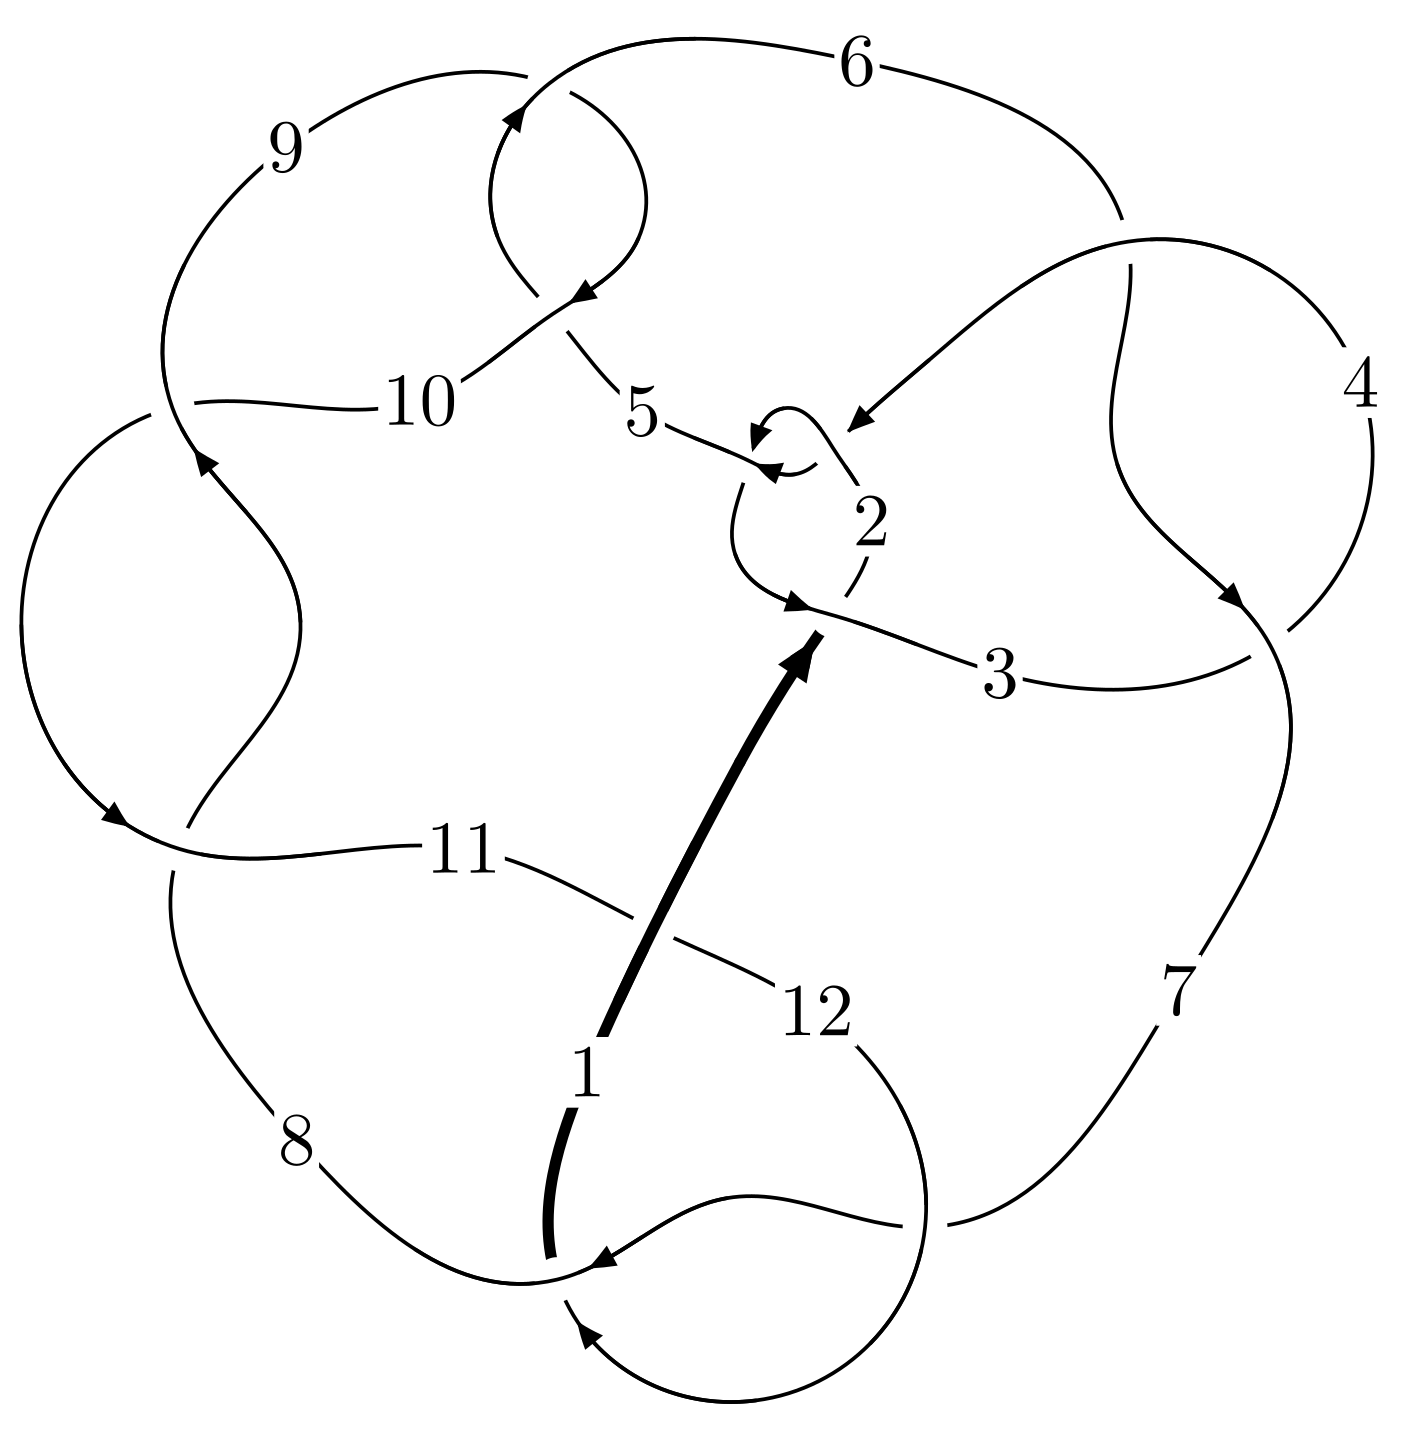
\includegraphics[width=112pt]{../../../GIT/diagram.site/Diagrams/png/855_12a_0054.png}\\
\ \ \ A knot diagram\footnotemark}&
\allowdisplaybreaks
\textbf{Linearized knot diagam} \\
\cline{2-2}
 &
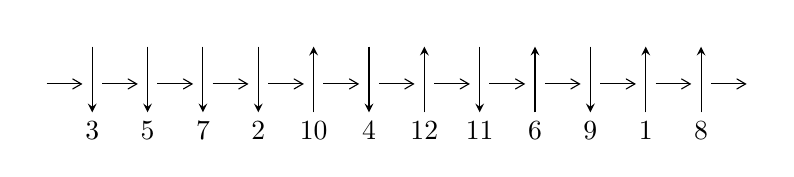
\begin{tikzpicture}[x=20pt, y=17pt]
	% nodes
	\node (C0) at (0, 0) {};
	\node (C1) at (1, 0) {};
	\node (C1U) at (1, +1) {};
	\node (C1D) at (1, -1) {3};

	\node (C2) at (2, 0) {};
	\node (C2U) at (2, +1) {};
	\node (C2D) at (2, -1) {5};

	\node (C3) at (3, 0) {};
	\node (C3U) at (3, +1) {};
	\node (C3D) at (3, -1) {7};

	\node (C4) at (4, 0) {};
	\node (C4U) at (4, +1) {};
	\node (C4D) at (4, -1) {2};

	\node (C5) at (5, 0) {};
	\node (C5U) at (5, +1) {};
	\node (C5D) at (5, -1) {10};

	\node (C6) at (6, 0) {};
	\node (C6U) at (6, +1) {};
	\node (C6D) at (6, -1) {4};

	\node (C7) at (7, 0) {};
	\node (C7U) at (7, +1) {};
	\node (C7D) at (7, -1) {12};

	\node (C8) at (8, 0) {};
	\node (C8U) at (8, +1) {};
	\node (C8D) at (8, -1) {11};

	\node (C9) at (9, 0) {};
	\node (C9U) at (9, +1) {};
	\node (C9D) at (9, -1) {6};

	\node (C10) at (10, 0) {};
	\node (C10U) at (10, +1) {};
	\node (C10D) at (10, -1) {9};

	\node (C11) at (11, 0) {};
	\node (C11U) at (11, +1) {};
	\node (C11D) at (11, -1) {1};

	\node (C12) at (12, 0) {};
	\node (C12U) at (12, +1) {};
	\node (C12D) at (12, -1) {8};
	\node (C13) at (13, 0) {};

	% arrows
	\draw[->,>={angle 60}]
	(C0) edge (C1) (C1) edge (C2) (C2) edge (C3) (C3) edge (C4) (C4) edge (C5) (C5) edge (C6) (C6) edge (C7) (C7) edge (C8) (C8) edge (C9) (C9) edge (C10) (C10) edge (C11) (C11) edge (C12) (C12) edge (C13) ;	\draw[->,>=stealth]
	(C1U) edge (C1D) (C2U) edge (C2D) (C3U) edge (C3D) (C4U) edge (C4D) (C5D) edge (C5U) (C6U) edge (C6D) (C7D) edge (C7U) (C8U) edge (C8D) (C9D) edge (C9U) (C10U) edge (C10D) (C11D) edge (C11U) (C12D) edge (C12U) ;
	\end{tikzpicture} \\
\hhline{~~} \\& 
\textbf{Solving Sequence} \\ \cline{2-2} 
 &
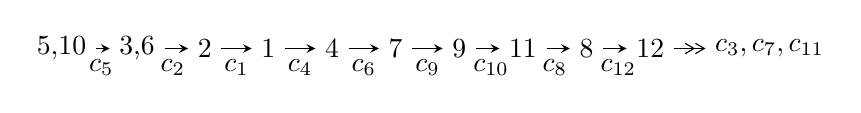
\begin{tikzpicture}[x=23pt, y=7pt]
	% node
	\node (A0) at (-1/8, 0) {5,10};
	\node (A1) at (17/16, 0) {3,6};
	\node (A2) at (17/8, 0) {2};
	\node (A3) at (25/8, 0) {1};
	\node (A4) at (33/8, 0) {4};
	\node (A5) at (41/8, 0) {7};
	\node (A6) at (49/8, 0) {9};
	\node (A7) at (57/8, 0) {11};
	\node (A8) at (65/8, 0) {8};
	\node (A9) at (73/8, 0) {12};
	\node (C1) at (1/2, -1) {$c_{5}$};
	\node (C2) at (13/8, -1) {$c_{2}$};
	\node (C3) at (21/8, -1) {$c_{1}$};
	\node (C4) at (29/8, -1) {$c_{4}$};
	\node (C5) at (37/8, -1) {$c_{6}$};
	\node (C6) at (45/8, -1) {$c_{9}$};
	\node (C7) at (53/8, -1) {$c_{10}$};
	\node (C8) at (61/8, -1) {$c_{8}$};
	\node (C9) at (69/8, -1) {$c_{12}$};
	\node (A10) at (11, 0) {$c_{3},c_{7},c_{11}$};

	% edge
	\draw[->,>=stealth]	
	(A0) edge (A1) (A1) edge (A2) (A2) edge (A3) (A3) edge (A4) (A4) edge (A5) (A5) edge (A6) (A6) edge (A7) (A7) edge (A8) (A8) edge (A9) ;
	\draw[->>,>={angle 60}]	
	(A9) edge (A10);
\end{tikzpicture} \\ 

\end{tabular} \\

\footnotetext{
The image of knot diagram is generated by the software ``\textbf{Draw programme}" developed by Andrew Bartholomew(\url{http://www.layer8.co.uk/maths/draw/index.htm\#Running-draw}), where we modified some parts for our purpose(\url{https://github.com/CATsTAILs/LinksPainter}).
}\phantom \\ \newline 
\centering \textbf{Ideals for irreducible components\footnotemark of $X_{\text{par}}$} 
 
\begin{align*}
I^u_{1}&=\langle 
1.70479\times10^{114} u^{95}-2.20755\times10^{114} u^{94}+\cdots+2.05537\times10^{115} b-3.80401\times10^{115},\\
\phantom{I^u_{1}}&\phantom{= \langle  }8.56716\times10^{113} u^{95}-4.40413\times10^{114} u^{94}+\cdots+4.11073\times10^{115} a+1.80283\times10^{116},\;u^{96}-2 u^{95}+\cdots-12 u-8\rangle \\
I^u_{2}&=\langle 
b+1,\;- u^8+2 u^7-3 u^6+3 u^5-4 u^4+4 u^3-3 u^2+a+2 u-1,\;u^9- u^8+2 u^7- u^6+3 u^5- u^4+2 u^3+u+1\rangle \\
\\
I^v_{1}&=\langle 
a,\;- v^2+b+3 v+1,\;v^3-2 v^2-3 v-1\rangle \\
\end{align*}
\raggedright * 3 irreducible components of $\dim_{\mathbb{C}}=0$, with total 108 representations.\\
\footnotetext{All coefficients of polynomials are rational numbers. But the coefficients are sometimes approximated in decimal forms when there is not enough margin.}
\newpage
\renewcommand{\arraystretch}{1}
\centering \section*{I. $I^u_{1}= \langle 1.70\times10^{114} u^{95}-2.21\times10^{114} u^{94}+\cdots+2.06\times10^{115} b-3.80\times10^{115},\;8.57\times10^{113} u^{95}-4.40\times10^{114} u^{94}+\cdots+4.11\times10^{115} a+1.80\times10^{116},\;u^{96}-2 u^{95}+\cdots-12 u-8 \rangle$}
\flushleft \textbf{(i) Arc colorings}\\
\begin{tabular}{m{7pt} m{180pt} m{7pt} m{180pt} }
\flushright $a_{5}=$&$\begin{pmatrix}1\\0\end{pmatrix}$ \\
\flushright $a_{10}=$&$\begin{pmatrix}0\\u\end{pmatrix}$ \\
\flushright $a_{3}=$&$\begin{pmatrix}-0.0208409 u^{95}+0.107137 u^{94}+\cdots-7.91306 u-4.38566\\-0.0829433 u^{95}+0.107404 u^{94}+\cdots+3.53916 u+1.85077\end{pmatrix}$ \\
\flushright $a_{6}=$&$\begin{pmatrix}1\\- u^2\end{pmatrix}$ \\
\flushright $a_{2}=$&$\begin{pmatrix}-0.103784 u^{95}+0.214541 u^{94}+\cdots-4.37390 u-2.53489\\-0.0829433 u^{95}+0.107404 u^{94}+\cdots+3.53916 u+1.85077\end{pmatrix}$ \\
\flushright $a_{1}=$&$\begin{pmatrix}0.0473624 u^{95}-0.0186442 u^{94}+\cdots-5.36990 u-2.42402\\-0.137727 u^{95}+0.287200 u^{94}+\cdots+2.40951 u-0.488149\end{pmatrix}$ \\
\flushright $a_{4}=$&$\begin{pmatrix}-0.213197 u^{95}+0.429416 u^{94}+\cdots-1.62144 u-0.459408\\0.0719032 u^{95}-0.0553870 u^{94}+\cdots-0.297884 u-2.76461\end{pmatrix}$ \\
\flushright $a_{7}=$&$\begin{pmatrix}-0.0903647 u^{95}+0.268555 u^{94}+\cdots-2.96038 u-2.91217\\0.199681 u^{95}-0.470810 u^{94}+\cdots-2.74051 u-0.214459\end{pmatrix}$ \\
\flushright $a_{9}=$&$\begin{pmatrix}- u\\u^3+u\end{pmatrix}$ \\
\flushright $a_{11}=$&$\begin{pmatrix}- u^3\\u^5+u^3+u\end{pmatrix}$ \\
\flushright $a_{8}=$&$\begin{pmatrix}- u^5- u\\u^7+u^5+2 u^3+u\end{pmatrix}$ \\
\flushright $a_{12}=$&$\begin{pmatrix}-0.0255767 u^{95}+0.0598845 u^{94}+\cdots-5.58218 u-3.51029\\0.00949794 u^{95}+0.0415095 u^{94}+\cdots+2.45224 u+0.0562999\end{pmatrix}$\\&\end{tabular}
\flushleft \textbf{(ii) Obstruction class $= -1$}\\~\\
\flushleft \textbf{(iii) Cusp Shapes $= -0.236170 u^{95}+0.601131 u^{94}+\cdots+0.772462 u-8.63749$}\\~\\
\newpage\renewcommand{\arraystretch}{1}
\flushleft \textbf{(iv) u-Polynomials at the component}\newline \\
\begin{tabular}{m{50pt}|m{274pt}}
Crossings & \hspace{64pt}u-Polynomials at each crossing \\
\hline $$\begin{aligned}c_{1}\end{aligned}$$&$\begin{aligned}
&u^{96}+41 u^{95}+\cdots+401 u+1
\end{aligned}$\\
\hline $$\begin{aligned}c_{2},c_{4}\end{aligned}$$&$\begin{aligned}
&u^{96}-11 u^{95}+\cdots+7 u+1
\end{aligned}$\\
\hline $$\begin{aligned}c_{3},c_{6}\end{aligned}$$&$\begin{aligned}
&u^{96}-2 u^{95}+\cdots+1536 u-512
\end{aligned}$\\
\hline $$\begin{aligned}c_{5},c_{9}\end{aligned}$$&$\begin{aligned}
&u^{96}-2 u^{95}+\cdots-12 u-8
\end{aligned}$\\
\hline $$\begin{aligned}c_{7},c_{12}\end{aligned}$$&$\begin{aligned}
&u^{96}+5 u^{95}+\cdots-8 u+1
\end{aligned}$\\
\hline $$\begin{aligned}c_{8},c_{10}\end{aligned}$$&$\begin{aligned}
&u^{96}+24 u^{95}+\cdots+48 u+64
\end{aligned}$\\
\hline $$\begin{aligned}c_{11}\end{aligned}$$&$\begin{aligned}
&u^{96}-55 u^{95}+\cdots-218 u+1
\end{aligned}$\\
\hline
\end{tabular}\\~\\
\newpage\renewcommand{\arraystretch}{1}
\flushleft \textbf{(v) Riley Polynomials at the component}\newline \\
\begin{tabular}{m{50pt}|m{274pt}}
Crossings & \hspace{64pt}Riley Polynomials at each crossing \\
\hline $$\begin{aligned}c_{1}\end{aligned}$$&$\begin{aligned}
&y^{96}+39 y^{95}+\cdots-140705 y+1
\end{aligned}$\\
\hline $$\begin{aligned}c_{2},c_{4}\end{aligned}$$&$\begin{aligned}
&y^{96}-41 y^{95}+\cdots-401 y+1
\end{aligned}$\\
\hline $$\begin{aligned}c_{3},c_{6}\end{aligned}$$&$\begin{aligned}
&y^{96}+60 y^{95}+\cdots+1835008 y+262144
\end{aligned}$\\
\hline $$\begin{aligned}c_{5},c_{9}\end{aligned}$$&$\begin{aligned}
&y^{96}+24 y^{95}+\cdots+48 y+64
\end{aligned}$\\
\hline $$\begin{aligned}c_{7},c_{12}\end{aligned}$$&$\begin{aligned}
&y^{96}-55 y^{95}+\cdots-218 y+1
\end{aligned}$\\
\hline $$\begin{aligned}c_{8},c_{10}\end{aligned}$$&$\begin{aligned}
&y^{96}+92 y^{95}+\cdots-879872 y+4096
\end{aligned}$\\
\hline $$\begin{aligned}c_{11}\end{aligned}$$&$\begin{aligned}
&y^{96}-23 y^{95}+\cdots-43342 y+1
\end{aligned}$\\
\hline
\end{tabular}\\~\\
\newpage\flushleft \textbf{(vi) Complex Volumes and Cusp Shapes}
$$\begin{array}{c|c|c}  
\text{Solutions to }I^u_{1}& \I (\text{vol} + \sqrt{-1}CS) & \text{Cusp shape}\\
 \hline 
\begin{aligned}
u &= -0.331849 + 0.953547 I \\
a &= -0.991852 + 0.187481 I \\
b &= -1.226360 + 0.183799 I\end{aligned}
 & -2.99925 - 3.60208 I & \phantom{-0.000000 } 0 \\ \hline\begin{aligned}
u &= -0.331849 - 0.953547 I \\
a &= -0.991852 - 0.187481 I \\
b &= -1.226360 - 0.183799 I\end{aligned}
 & -2.99925 + 3.60208 I & \phantom{-0.000000 } 0 \\ \hline\begin{aligned}
u &= \phantom{-}0.420726 + 0.894455 I \\
a &= \phantom{-}0.0748654 + 0.0783523 I \\
b &= \phantom{-}0.326390 + 0.493463 I\end{aligned}
 & -0.09751 + 2.03694 I & \phantom{-0.000000 } 0 \\ \hline\begin{aligned}
u &= \phantom{-}0.420726 - 0.894455 I \\
a &= \phantom{-}0.0748654 - 0.0783523 I \\
b &= \phantom{-}0.326390 - 0.493463 I\end{aligned}
 & -0.09751 - 2.03694 I & \phantom{-0.000000 } 0 \\ \hline\begin{aligned}
u &= -0.763608 + 0.666822 I \\
a &= \phantom{-}0.370790 - 0.523796 I \\
b &= \phantom{-}0.479897 + 0.066967 I\end{aligned}
 & \phantom{-}3.69919 + 1.25518 I & \phantom{-0.000000 } 0 \\ \hline\begin{aligned}
u &= -0.763608 - 0.666822 I \\
a &= \phantom{-}0.370790 + 0.523796 I \\
b &= \phantom{-}0.479897 - 0.066967 I\end{aligned}
 & \phantom{-}3.69919 - 1.25518 I & \phantom{-0.000000 } 0 \\ \hline\begin{aligned}
u &= -0.917832 + 0.330602 I \\
a &= -0.422961 + 0.922598 I \\
b &= \phantom{-}1.011070 - 0.616866 I\end{aligned}
 & \phantom{-}2.58601 + 6.51221 I & \phantom{-0.000000 } 0 \\ \hline\begin{aligned}
u &= -0.917832 - 0.330602 I \\
a &= -0.422961 - 0.922598 I \\
b &= \phantom{-}1.011070 + 0.616866 I\end{aligned}
 & \phantom{-}2.58601 - 6.51221 I & \phantom{-0.000000 } 0 \\ \hline\begin{aligned}
u &= -0.846687 + 0.463347 I \\
a &= \phantom{-}0.080098 - 1.096030 I \\
b &= \phantom{-}0.571760 + 0.611302 I\end{aligned}
 & \phantom{-}3.84701 + 1.59882 I & \phantom{-0.000000 } 0 \\ \hline\begin{aligned}
u &= -0.846687 - 0.463347 I \\
a &= \phantom{-}0.080098 + 1.096030 I \\
b &= \phantom{-}0.571760 - 0.611302 I\end{aligned}
 & \phantom{-}3.84701 - 1.59882 I & \phantom{-0.000000 } 0\\
 \hline 
 \end{array}$$\newpage$$\begin{array}{c|c|c}  
\text{Solutions to }I^u_{1}& \I (\text{vol} + \sqrt{-1}CS) & \text{Cusp shape}\\
 \hline 
\begin{aligned}
u &= -0.214407 + 0.917724 I \\
a &= -1.21899 + 1.73083 I \\
b &= -1.043700 - 0.362721 I\end{aligned}
 & -3.72115 - 1.69356 I & -8.89200 + 0. I\phantom{ +0.000000I} \\ \hline\begin{aligned}
u &= -0.214407 - 0.917724 I \\
a &= -1.21899 - 1.73083 I \\
b &= -1.043700 + 0.362721 I\end{aligned}
 & -3.72115 + 1.69356 I & -8.89200 + 0. I\phantom{ +0.000000I} \\ \hline\begin{aligned}
u &= \phantom{-}0.399586 + 0.985773 I \\
a &= -0.64535 - 1.97533 I \\
b &= -1.015690 + 0.459888 I\end{aligned}
 & -2.29930 + 5.98929 I & \phantom{-0.000000 } 0 \\ \hline\begin{aligned}
u &= \phantom{-}0.399586 - 0.985773 I \\
a &= -0.64535 + 1.97533 I \\
b &= -1.015690 - 0.459888 I\end{aligned}
 & -2.29930 - 5.98929 I & \phantom{-0.000000 } 0 \\ \hline\begin{aligned}
u &= \phantom{-}0.105934 + 0.913879 I \\
a &= -1.49280 + 0.48603 I \\
b &= -1.144490 - 0.244528 I\end{aligned}
 & -4.04166 - 0.52516 I & -8.55610 + 0. I\phantom{ +0.000000I} \\ \hline\begin{aligned}
u &= \phantom{-}0.105934 - 0.913879 I \\
a &= -1.49280 - 0.48603 I \\
b &= -1.144490 + 0.244528 I\end{aligned}
 & -4.04166 + 0.52516 I & -8.55610 + 0. I\phantom{ +0.000000I} \\ \hline\begin{aligned}
u &= \phantom{-}0.543375 + 0.935475 I \\
a &= \phantom{-}0.306378 + 0.400786 I \\
b &= \phantom{-}0.588526 + 0.269748 I\end{aligned}
 & -0.07900 + 2.11206 I & \phantom{-0.000000 } 0 \\ \hline\begin{aligned}
u &= \phantom{-}0.543375 - 0.935475 I \\
a &= \phantom{-}0.306378 - 0.400786 I \\
b &= \phantom{-}0.588526 - 0.269748 I\end{aligned}
 & -0.07900 - 2.11206 I & \phantom{-0.000000 } 0 \\ \hline\begin{aligned}
u &= \phantom{-}0.287889 + 0.845646 I \\
a &= \phantom{-}0.949105 + 0.732014 I \\
b &= -0.483494 - 0.489887 I\end{aligned}
 & -0.67980 + 2.01844 I & -2.00000 - 3.46901 I \\ \hline\begin{aligned}
u &= \phantom{-}0.287889 - 0.845646 I \\
a &= \phantom{-}0.949105 - 0.732014 I \\
b &= -0.483494 + 0.489887 I\end{aligned}
 & -0.67980 - 2.01844 I & -2.00000 + 3.46901 I\\
 \hline 
 \end{array}$$\newpage$$\begin{array}{c|c|c}  
\text{Solutions to }I^u_{1}& \I (\text{vol} + \sqrt{-1}CS) & \text{Cusp shape}\\
 \hline 
\begin{aligned}
u &= \phantom{-}0.002493 + 1.116370 I \\
a &= \phantom{-}1.228320 + 0.018327 I \\
b &= \phantom{-}0.949803 - 0.482210 I\end{aligned}
 & -3.12502 + 4.24954 I & \phantom{-0.000000 } 0 \\ \hline\begin{aligned}
u &= \phantom{-}0.002493 - 1.116370 I \\
a &= \phantom{-}1.228320 - 0.018327 I \\
b &= \phantom{-}0.949803 + 0.482210 I\end{aligned}
 & -3.12502 - 4.24954 I & \phantom{-0.000000 } 0 \\ \hline\begin{aligned}
u &= -0.508460 + 0.999100 I \\
a &= -0.361486 + 0.232503 I \\
b &= \phantom{-}0.336484 - 0.738021 I\end{aligned}
 & \phantom{-}1.95677 - 6.48071 I & \phantom{-0.000000 } 0 \\ \hline\begin{aligned}
u &= -0.508460 - 0.999100 I \\
a &= -0.361486 - 0.232503 I \\
b &= \phantom{-}0.336484 + 0.738021 I\end{aligned}
 & \phantom{-}1.95677 + 6.48071 I & \phantom{-0.000000 } 0 \\ \hline\begin{aligned}
u &= -0.416500 + 0.770558 I \\
a &= -0.483230 - 1.295950 I \\
b &= \phantom{-}0.671787 - 0.640819 I\end{aligned}
 & \phantom{-}4.46916 + 0.68945 I & \phantom{-}3.28117 + 0.85960 I \\ \hline\begin{aligned}
u &= -0.416500 - 0.770558 I \\
a &= -0.483230 + 1.295950 I \\
b &= \phantom{-}0.671787 + 0.640819 I\end{aligned}
 & \phantom{-}4.46916 - 0.68945 I & \phantom{-}3.28117 - 0.85960 I \\ \hline\begin{aligned}
u &= \phantom{-}0.332265 + 1.076590 I \\
a &= \phantom{-}1.42109 + 1.04142 I \\
b &= \phantom{-}1.046100 - 0.573034 I\end{aligned}
 & -1.83045 + 6.55518 I & \phantom{-0.000000 } 0 \\ \hline\begin{aligned}
u &= \phantom{-}0.332265 - 1.076590 I \\
a &= \phantom{-}1.42109 - 1.04142 I \\
b &= \phantom{-}1.046100 + 0.573034 I\end{aligned}
 & -1.83045 - 6.55518 I & \phantom{-0.000000 } 0 \\ \hline\begin{aligned}
u &= \phantom{-}0.177267 + 1.115030 I \\
a &= \phantom{-}0.907127 + 0.317756 I \\
b &= \phantom{-}0.879589 + 0.432826 I\end{aligned}
 & -2.75506 + 0.64484 I & \phantom{-0.000000 } 0 \\ \hline\begin{aligned}
u &= \phantom{-}0.177267 - 1.115030 I \\
a &= \phantom{-}0.907127 - 0.317756 I \\
b &= \phantom{-}0.879589 - 0.432826 I\end{aligned}
 & -2.75506 - 0.64484 I & \phantom{-0.000000 } 0\\
 \hline 
 \end{array}$$\newpage$$\begin{array}{c|c|c}  
\text{Solutions to }I^u_{1}& \I (\text{vol} + \sqrt{-1}CS) & \text{Cusp shape}\\
 \hline 
\begin{aligned}
u &= -0.247496 + 0.816258 I \\
a &= \phantom{-}2.79839 - 0.99348 I \\
b &= \phantom{-}0.969526 + 0.629311 I\end{aligned}
 & \phantom{-}3.58367 - 4.30558 I & -0.11915 + 6.48044 I \\ \hline\begin{aligned}
u &= -0.247496 - 0.816258 I \\
a &= \phantom{-}2.79839 + 0.99348 I \\
b &= \phantom{-}0.969526 - 0.629311 I\end{aligned}
 & \phantom{-}3.58367 + 4.30558 I & -0.11915 - 6.48044 I \\ \hline\begin{aligned}
u &= \phantom{-}0.840798 + 0.068830 I \\
a &= -0.306920 - 0.930091 I \\
b &= \phantom{-}0.918979 + 0.594287 I\end{aligned}
 & \phantom{-}1.56693 - 2.64898 I & -0.12373 + 1.94416 I \\ \hline\begin{aligned}
u &= \phantom{-}0.840798 - 0.068830 I \\
a &= -0.306920 + 0.930091 I \\
b &= \phantom{-}0.918979 - 0.594287 I\end{aligned}
 & \phantom{-}1.56693 + 2.64898 I & -0.12373 - 1.94416 I \\ \hline\begin{aligned}
u &= \phantom{-}0.039988 + 0.842192 I \\
a &= \phantom{-}0.669881 - 0.384390 I \\
b &= -0.173785 + 0.414358 I\end{aligned}
 & -1.31139 + 1.53275 I & -3.91456 - 5.18456 I \\ \hline\begin{aligned}
u &= \phantom{-}0.039988 - 0.842192 I \\
a &= \phantom{-}0.669881 + 0.384390 I \\
b &= -0.173785 - 0.414358 I\end{aligned}
 & -1.31139 - 1.53275 I & -3.91456 + 5.18456 I \\ \hline\begin{aligned}
u &= \phantom{-}0.799059 + 0.846331 I \\
a &= \phantom{-}1.07319 + 1.14008 I \\
b &= -0.806160 - 0.624229 I\end{aligned}
 & \phantom{-}2.43670 + 0.52493 I & \phantom{-0.000000 } 0 \\ \hline\begin{aligned}
u &= \phantom{-}0.799059 - 0.846331 I \\
a &= \phantom{-}1.07319 - 1.14008 I \\
b &= -0.806160 + 0.624229 I\end{aligned}
 & \phantom{-}2.43670 - 0.52493 I & \phantom{-0.000000 } 0 \\ \hline\begin{aligned}
u &= -0.767472 + 0.888370 I \\
a &= -0.084906 + 0.851187 I \\
b &= -1.332930 + 0.034727 I\end{aligned}
 & \phantom{-}0.72602 - 2.90143 I & \phantom{-0.000000 } 0 \\ \hline\begin{aligned}
u &= -0.767472 - 0.888370 I \\
a &= -0.084906 - 0.851187 I \\
b &= -1.332930 - 0.034727 I\end{aligned}
 & \phantom{-}0.72602 + 2.90143 I & \phantom{-0.000000 } 0\\
 \hline 
 \end{array}$$\newpage$$\begin{array}{c|c|c}  
\text{Solutions to }I^u_{1}& \I (\text{vol} + \sqrt{-1}CS) & \text{Cusp shape}\\
 \hline 
\begin{aligned}
u &= -0.885713 + 0.776635 I \\
a &= -0.572131 + 1.015580 I \\
b &= \phantom{-}1.108900 - 0.724154 I\end{aligned}
 & \phantom{-}6.26538 + 5.58089 I & \phantom{-0.000000 } 0 \\ \hline\begin{aligned}
u &= -0.885713 - 0.776635 I \\
a &= -0.572131 - 1.015580 I \\
b &= \phantom{-}1.108900 + 0.724154 I\end{aligned}
 & \phantom{-}6.26538 - 5.58089 I & \phantom{-0.000000 } 0 \\ \hline\begin{aligned}
u &= \phantom{-}0.857556 + 0.825746 I \\
a &= \phantom{-}0.080065 - 0.973811 I \\
b &= -1.340690 + 0.009120 I\end{aligned}
 & \phantom{-}4.57395 - 1.45279 I & \phantom{-0.000000 } 0 \\ \hline\begin{aligned}
u &= \phantom{-}0.857556 - 0.825746 I \\
a &= \phantom{-}0.080065 + 0.973811 I \\
b &= -1.340690 - 0.009120 I\end{aligned}
 & \phantom{-}4.57395 + 1.45279 I & \phantom{-0.000000 } 0 \\ \hline\begin{aligned}
u &= \phantom{-}0.830770 + 0.862931 I \\
a &= -0.586564 - 1.051620 I \\
b &= \phantom{-}1.112920 + 0.756547 I\end{aligned}
 & \phantom{-}10.10790 - 1.19035 I & \phantom{-0.000000 } 0 \\ \hline\begin{aligned}
u &= \phantom{-}0.830770 - 0.862931 I \\
a &= -0.586564 + 1.051620 I \\
b &= \phantom{-}1.112920 - 0.756547 I\end{aligned}
 & \phantom{-}10.10790 + 1.19035 I & \phantom{-0.000000 } 0 \\ \hline\begin{aligned}
u &= \phantom{-}0.760213 + 0.255609 I \\
a &= -0.148446 + 1.002920 I \\
b &= \phantom{-}0.776189 - 0.607942 I\end{aligned}
 & \phantom{-}2.00761 + 2.10017 I & \phantom{-}0.83891 - 4.53868 I \\ \hline\begin{aligned}
u &= \phantom{-}0.760213 - 0.255609 I \\
a &= -0.148446 - 1.002920 I \\
b &= \phantom{-}0.776189 + 0.607942 I\end{aligned}
 & \phantom{-}2.00761 - 2.10017 I & \phantom{-}0.83891 + 4.53868 I \\ \hline\begin{aligned}
u &= -0.838980 + 0.859841 I \\
a &= \phantom{-}0.17172 + 2.31211 I \\
b &= -0.839704 - 0.634470 I\end{aligned}
 & \phantom{-}6.20074 - 1.00773 I & \phantom{-0.000000 } 0 \\ \hline\begin{aligned}
u &= -0.838980 - 0.859841 I \\
a &= \phantom{-}0.17172 - 2.31211 I \\
b &= -0.839704 + 0.634470 I\end{aligned}
 & \phantom{-}6.20074 + 1.00773 I & \phantom{-0.000000 } 0\\
 \hline 
 \end{array}$$\newpage$$\begin{array}{c|c|c}  
\text{Solutions to }I^u_{1}& \I (\text{vol} + \sqrt{-1}CS) & \text{Cusp shape}\\
 \hline 
\begin{aligned}
u &= -0.474625 + 1.104840 I \\
a &= \phantom{-}1.12838 - 1.39898 I \\
b &= \phantom{-}1.091600 + 0.599495 I\end{aligned}
 & -0.12483 - 11.51150 I & \phantom{-0.000000 } 0 \\ \hline\begin{aligned}
u &= -0.474625 - 1.104840 I \\
a &= \phantom{-}1.12838 + 1.39898 I \\
b &= \phantom{-}1.091600 - 0.599495 I\end{aligned}
 & -0.12483 + 11.51150 I & \phantom{-0.000000 } 0 \\ \hline\begin{aligned}
u &= -0.870715 + 0.833568 I \\
a &= -0.05442 - 1.45713 I \\
b &= \phantom{-}0.556085 + 0.944376 I\end{aligned}
 & \phantom{-}7.96094 - 0.52062 I & \phantom{-0.000000 } 0 \\ \hline\begin{aligned}
u &= -0.870715 - 0.833568 I \\
a &= -0.05442 + 1.45713 I \\
b &= \phantom{-}0.556085 - 0.944376 I\end{aligned}
 & \phantom{-}7.96094 + 0.52062 I & \phantom{-0.000000 } 0 \\ \hline\begin{aligned}
u &= -0.894404 + 0.820640 I \\
a &= \phantom{-}1.08831 - 1.18593 I \\
b &= -0.861586 + 0.633055 I\end{aligned}
 & \phantom{-}6.13236 + 3.94857 I & \phantom{-0.000000 } 0 \\ \hline\begin{aligned}
u &= -0.894404 - 0.820640 I \\
a &= \phantom{-}1.08831 + 1.18593 I \\
b &= -0.861586 - 0.633055 I\end{aligned}
 & \phantom{-}6.13236 - 3.94857 I & \phantom{-0.000000 } 0 \\ \hline\begin{aligned}
u &= \phantom{-}0.781161 + 0.930558 I \\
a &= \phantom{-}0.06641 - 2.24202 I \\
b &= -0.888865 + 0.621738 I\end{aligned}
 & \phantom{-}2.17830 + 5.41664 I & \phantom{-0.000000 } 0 \\ \hline\begin{aligned}
u &= \phantom{-}0.781161 - 0.930558 I \\
a &= \phantom{-}0.06641 + 2.24202 I \\
b &= -0.888865 - 0.621738 I\end{aligned}
 & \phantom{-}2.17830 - 5.41664 I & \phantom{-0.000000 } 0 \\ \hline\begin{aligned}
u &= \phantom{-}0.806984 + 0.930820 I \\
a &= \phantom{-}0.56083 + 2.34249 I \\
b &= \phantom{-}1.126410 - 0.722210 I\end{aligned}
 & \phantom{-}9.89480 + 7.30761 I & \phantom{-0.000000 } 0 \\ \hline\begin{aligned}
u &= \phantom{-}0.806984 - 0.930820 I \\
a &= \phantom{-}0.56083 - 2.34249 I \\
b &= \phantom{-}1.126410 + 0.722210 I\end{aligned}
 & \phantom{-}9.89480 - 7.30761 I & \phantom{-0.000000 } 0\\
 \hline 
 \end{array}$$\newpage$$\begin{array}{c|c|c}  
\text{Solutions to }I^u_{1}& \I (\text{vol} + \sqrt{-1}CS) & \text{Cusp shape}\\
 \hline 
\begin{aligned}
u &= -0.703854 + 1.011630 I \\
a &= \phantom{-}0.305278 - 0.370471 I \\
b &= \phantom{-}0.679665 - 0.142081 I\end{aligned}
 & \phantom{-}2.66867 - 6.83395 I & \phantom{-0.000000 } 0 \\ \hline\begin{aligned}
u &= -0.703854 - 1.011630 I \\
a &= \phantom{-}0.305278 + 0.370471 I \\
b &= \phantom{-}0.679665 + 0.142081 I\end{aligned}
 & \phantom{-}2.66867 + 6.83395 I & \phantom{-0.000000 } 0 \\ \hline\begin{aligned}
u &= \phantom{-}0.703787 + 0.300436 I \\
a &= \phantom{-}1.45363 + 1.29987 I \\
b &= -0.925873 - 0.325878 I\end{aligned}
 & -0.02370 - 2.00842 I & -1.62743 + 4.29984 I \\ \hline\begin{aligned}
u &= \phantom{-}0.703787 - 0.300436 I \\
a &= \phantom{-}1.45363 - 1.29987 I \\
b &= -0.925873 + 0.325878 I\end{aligned}
 & -0.02370 + 2.00842 I & -1.62743 - 4.29984 I \\ \hline\begin{aligned}
u &= \phantom{-}0.846783 + 0.902988 I \\
a &= -0.09596 + 1.47858 I \\
b &= \phantom{-}0.583726 - 0.977505 I\end{aligned}
 & \phantom{-}11.73460 + 5.11833 I & \phantom{-0.000000 } 0 \\ \hline\begin{aligned}
u &= \phantom{-}0.846783 - 0.902988 I \\
a &= -0.09596 - 1.47858 I \\
b &= \phantom{-}0.583726 + 0.977505 I\end{aligned}
 & \phantom{-}11.73460 - 5.11833 I & \phantom{-0.000000 } 0 \\ \hline\begin{aligned}
u &= -0.812021 + 0.937351 I \\
a &= \phantom{-}1.02775 - 1.15508 I \\
b &= -0.792949 + 0.675723 I\end{aligned}
 & \phantom{-}5.95824 - 5.15041 I & \phantom{-0.000000 } 0 \\ \hline\begin{aligned}
u &= -0.812021 - 0.937351 I \\
a &= \phantom{-}1.02775 + 1.15508 I \\
b &= -0.792949 - 0.675723 I\end{aligned}
 & \phantom{-}5.95824 + 5.15041 I & \phantom{-0.000000 } 0 \\ \hline\begin{aligned}
u &= \phantom{-}0.844920 + 0.911321 I \\
a &= -1.228240 - 0.696496 I \\
b &= \phantom{-}0.535424 + 0.960203 I\end{aligned}
 & \phantom{-}11.70970 + 1.16815 I & \phantom{-0.000000 } 0 \\ \hline\begin{aligned}
u &= \phantom{-}0.844920 - 0.911321 I \\
a &= -1.228240 + 0.696496 I \\
b &= \phantom{-}0.535424 - 0.960203 I\end{aligned}
 & \phantom{-}11.70970 - 1.16815 I & \phantom{-0.000000 } 0\\
 \hline 
 \end{array}$$\newpage$$\begin{array}{c|c|c}  
\text{Solutions to }I^u_{1}& \I (\text{vol} + \sqrt{-1}CS) & \text{Cusp shape}\\
 \hline 
\begin{aligned}
u &= \phantom{-}0.938146 + 0.839572 I \\
a &= -0.02587 + 1.49281 I \\
b &= \phantom{-}0.518746 - 0.964023 I\end{aligned}
 & \phantom{-}11.59380 - 4.19583 I & \phantom{-0.000000 } 0 \\ \hline\begin{aligned}
u &= \phantom{-}0.938146 - 0.839572 I \\
a &= -0.02587 - 1.49281 I \\
b &= \phantom{-}0.518746 + 0.964023 I\end{aligned}
 & \phantom{-}11.59380 + 4.19583 I & \phantom{-0.000000 } 0 \\ \hline\begin{aligned}
u &= \phantom{-}0.964249 + 0.810539 I \\
a &= -0.600574 - 0.998151 I \\
b &= \phantom{-}1.135580 + 0.716044 I\end{aligned}
 & \phantom{-}9.6993 - 10.3238 I & \phantom{-0.000000 } 0 \\ \hline\begin{aligned}
u &= \phantom{-}0.964249 - 0.810539 I \\
a &= -0.600574 + 0.998151 I \\
b &= \phantom{-}1.135580 - 0.716044 I\end{aligned}
 & \phantom{-}9.6993 + 10.3238 I & \phantom{-0.000000 } 0 \\ \hline\begin{aligned}
u &= \phantom{-}0.807188 + 0.967313 I \\
a &= \phantom{-}0.010286 - 0.719507 I \\
b &= -1.367010 - 0.045646 I\end{aligned}
 & \phantom{-}4.13276 + 7.64866 I & \phantom{-0.000000 } 0 \\ \hline\begin{aligned}
u &= \phantom{-}0.807188 - 0.967313 I \\
a &= \phantom{-}0.010286 + 0.719507 I \\
b &= -1.367010 + 0.045646 I\end{aligned}
 & \phantom{-}4.13276 - 7.64866 I & \phantom{-0.000000 } 0 \\ \hline\begin{aligned}
u &= -0.818771 + 0.967967 I \\
a &= -1.077720 + 0.692980 I \\
b &= \phantom{-}0.495683 - 0.960350 I\end{aligned}
 & \phantom{-}7.53995 - 5.75065 I & \phantom{-0.000000 } 0 \\ \hline\begin{aligned}
u &= -0.818771 - 0.967967 I \\
a &= -1.077720 - 0.692980 I \\
b &= \phantom{-}0.495683 + 0.960350 I\end{aligned}
 & \phantom{-}7.53995 + 5.75065 I & \phantom{-0.000000 } 0 \\ \hline\begin{aligned}
u &= -0.374478 + 0.621105 I \\
a &= -0.250485 - 1.236750 I \\
b &= \phantom{-}0.790669 + 0.824031 I\end{aligned}
 & \phantom{-}4.94910 - 3.81882 I & \phantom{-}2.10350 + 10.02722 I \\ \hline\begin{aligned}
u &= -0.374478 - 0.621105 I \\
a &= -0.250485 + 1.236750 I \\
b &= \phantom{-}0.790669 - 0.824031 I\end{aligned}
 & \phantom{-}4.94910 + 3.81882 I & \phantom{-}2.10350 - 10.02722 I\\
 \hline 
 \end{array}$$\newpage$$\begin{array}{c|c|c}  
\text{Solutions to }I^u_{1}& \I (\text{vol} + \sqrt{-1}CS) & \text{Cusp shape}\\
 \hline 
\begin{aligned}
u &= -0.798420 + 1.005590 I \\
a &= \phantom{-}0.54011 - 2.13936 I \\
b &= \phantom{-}1.143510 + 0.704102 I\end{aligned}
 & \phantom{-}5.55281 - 11.82450 I & \phantom{-0.000000 } 0 \\ \hline\begin{aligned}
u &= -0.798420 - 1.005590 I \\
a &= \phantom{-}0.54011 + 2.13936 I \\
b &= \phantom{-}1.143510 - 0.704102 I\end{aligned}
 & \phantom{-}5.55281 + 11.82450 I & \phantom{-0.000000 } 0 \\ \hline\begin{aligned}
u &= -0.822932 + 0.988050 I \\
a &= \phantom{-}0.10986 + 2.15970 I \\
b &= -0.907528 - 0.655336 I\end{aligned}
 & \phantom{-}5.60270 - 10.30350 I & \phantom{-0.000000 } 0 \\ \hline\begin{aligned}
u &= -0.822932 - 0.988050 I \\
a &= \phantom{-}0.10986 - 2.15970 I \\
b &= -0.907528 + 0.655336 I\end{aligned}
 & \phantom{-}5.60270 + 10.30350 I & \phantom{-0.000000 } 0 \\ \hline\begin{aligned}
u &= \phantom{-}0.852797 + 1.004360 I \\
a &= -1.040640 - 0.796571 I \\
b &= \phantom{-}0.485399 + 0.990678 I\end{aligned}
 & \phantom{-}11.0580 + 10.7846 I & \phantom{-0.000000 } 0 \\ \hline\begin{aligned}
u &= \phantom{-}0.852797 - 1.004360 I \\
a &= -1.040640 + 0.796571 I \\
b &= \phantom{-}0.485399 - 0.990678 I\end{aligned}
 & \phantom{-}11.0580 - 10.7846 I & \phantom{-0.000000 } 0 \\ \hline\begin{aligned}
u &= \phantom{-}0.846509 + 1.032650 I \\
a &= \phantom{-}0.40884 + 2.10501 I \\
b &= \phantom{-}1.160850 - 0.710725 I\end{aligned}
 & \phantom{-}8.9763 + 16.9659 I & \phantom{-0.000000 } 0 \\ \hline\begin{aligned}
u &= \phantom{-}0.846509 - 1.032650 I \\
a &= \phantom{-}0.40884 - 2.10501 I \\
b &= \phantom{-}1.160850 + 0.710725 I\end{aligned}
 & \phantom{-}8.9763 - 16.9659 I & \phantom{-0.000000 } 0 \\ \hline\begin{aligned}
u &= -0.593118 + 0.166075 I \\
a &= \phantom{-}1.21211 + 2.60731 I \\
b &= -1.065150 - 0.117254 I\end{aligned}
 & -0.593809 + 0.331522 I & \phantom{-}1.43748 - 9.72886 I \\ \hline\begin{aligned}
u &= -0.593118 - 0.166075 I \\
a &= \phantom{-}1.21211 - 2.60731 I \\
b &= -1.065150 + 0.117254 I\end{aligned}
 & -0.593809 - 0.331522 I & \phantom{-}1.43748 + 9.72886 I\\
 \hline 
 \end{array}$$\newpage$$\begin{array}{c|c|c}  
\text{Solutions to }I^u_{1}& \I (\text{vol} + \sqrt{-1}CS) & \text{Cusp shape}\\
 \hline 
\begin{aligned}
u &= -0.254616 + 0.556672 I \\
a &= -0.397794 + 1.141700 I \\
b &= \phantom{-}0.937472 - 0.785999 I\end{aligned}
 & \phantom{-}4.51649 + 2.17388 I & -1.65157 + 5.92574 I \\ \hline\begin{aligned}
u &= -0.254616 - 0.556672 I \\
a &= -0.397794 - 1.141700 I \\
b &= \phantom{-}0.937472 + 0.785999 I\end{aligned}
 & \phantom{-}4.51649 - 2.17388 I & -1.65157 - 5.92574 I \\ \hline\begin{aligned}
u &= \phantom{-}0.265888 + 0.464329 I \\
a &= -2.42948 - 5.30179 I \\
b &= -0.833958 + 0.214787 I\end{aligned}
 & \phantom{-}0.614687 + 0.409343 I & -5.88588 - 9.56935 I \\ \hline\begin{aligned}
u &= \phantom{-}0.265888 - 0.464329 I \\
a &= -2.42948 + 5.30179 I \\
b &= -0.833958 - 0.214787 I\end{aligned}
 & \phantom{-}0.614687 - 0.409343 I & -5.88588 + 9.56935 I \\ \hline\begin{aligned}
u &= \phantom{-}0.463872\phantom{ +0.000000I} \\
a &= \phantom{-}1.34884\phantom{ +0.000000I} \\
b &= -0.0516319\phantom{ +0.000000I}\end{aligned}
 & \phantom{-}1.25812\phantom{ +0.000000I} & \phantom{-}8.69990\phantom{ +0.000000I} \\ \hline\begin{aligned}
u &= -0.262621\phantom{ +0.000000I} \\
a &= \phantom{-}2.59919\phantom{ +0.000000I} \\
b &= -0.826000\phantom{ +0.000000I}\end{aligned}
 & -1.19847\phantom{ +0.000000I} & -8.67400\phantom{ +0.000000I}\\
 \hline 
 \end{array}$$\newpage\newpage\renewcommand{\arraystretch}{1}
\centering \section*{II. $I^u_{2}= \langle b+1,\;- u^8+2 u^7+\cdots+a-1,\;u^9- u^8+2 u^7- u^6+3 u^5- u^4+2 u^3+u+1 \rangle$}
\flushleft \textbf{(i) Arc colorings}\\
\begin{tabular}{m{7pt} m{180pt} m{7pt} m{180pt} }
\flushright $a_{5}=$&$\begin{pmatrix}1\\0\end{pmatrix}$ \\
\flushright $a_{10}=$&$\begin{pmatrix}0\\u\end{pmatrix}$ \\
\flushright $a_{3}=$&$\begin{pmatrix}u^8-2 u^7+3 u^6-3 u^5+4 u^4-4 u^3+3 u^2-2 u+1\\-1\end{pmatrix}$ \\
\flushright $a_{6}=$&$\begin{pmatrix}1\\- u^2\end{pmatrix}$ \\
\flushright $a_{2}=$&$\begin{pmatrix}u^8-2 u^7+3 u^6-3 u^5+4 u^4-4 u^3+3 u^2-2 u\\-1\end{pmatrix}$ \\
\flushright $a_{1}=$&$\begin{pmatrix}-1\\0\end{pmatrix}$ \\
\flushright $a_{4}=$&$\begin{pmatrix}u^8-2 u^7+3 u^6-3 u^5+4 u^4-4 u^3+3 u^2-2 u+1\\-1\end{pmatrix}$ \\
\flushright $a_{7}=$&$\begin{pmatrix}1\\- u^2\end{pmatrix}$ \\
\flushright $a_{9}=$&$\begin{pmatrix}- u\\u^3+u\end{pmatrix}$ \\
\flushright $a_{11}=$&$\begin{pmatrix}- u^3\\u^5+u^3+u\end{pmatrix}$ \\
\flushright $a_{8}=$&$\begin{pmatrix}- u^5- u\\u^7+u^5+2 u^3+u\end{pmatrix}$ \\
\flushright $a_{12}=$&$\begin{pmatrix}u^5+u\\u^5+u^3+u\end{pmatrix}$\\&\end{tabular}
\flushleft \textbf{(ii) Obstruction class $= 1$}\\~\\
\flushleft \textbf{(iii) Cusp Shapes $= 3 u^8-8 u^7+12 u^6-11 u^5+18 u^4-17 u^3+15 u^2-6 u+4$}\\~\\
\newpage\renewcommand{\arraystretch}{1}
\flushleft \textbf{(iv) u-Polynomials at the component}\newline \\
\begin{tabular}{m{50pt}|m{274pt}}
Crossings & \hspace{64pt}u-Polynomials at each crossing \\
\hline $$\begin{aligned}c_{1},c_{2}\end{aligned}$$&$\begin{aligned}
&(u-1)^9
\end{aligned}$\\
\hline $$\begin{aligned}c_{3},c_{6}\end{aligned}$$&$\begin{aligned}
&u^9
\end{aligned}$\\
\hline $$\begin{aligned}c_{4}\end{aligned}$$&$\begin{aligned}
&(u+1)^9
\end{aligned}$\\
\hline $$\begin{aligned}c_{5}\end{aligned}$$&$\begin{aligned}
&u^9- u^8+2 u^7- u^6+3 u^5- u^4+2 u^3+u+1
\end{aligned}$\\
\hline $$\begin{aligned}c_{7}\end{aligned}$$&$\begin{aligned}
&u^9- u^8-2 u^7+3 u^6+u^5-3 u^4+2 u^3- u+1
\end{aligned}$\\
\hline $$\begin{aligned}c_{8}\end{aligned}$$&$\begin{aligned}
&u^9-3 u^8+8 u^7-13 u^6+17 u^5-17 u^4+12 u^3-6 u^2+u+1
\end{aligned}$\\
\hline $$\begin{aligned}c_{9}\end{aligned}$$&$\begin{aligned}
&u^9+u^8+2 u^7+u^6+3 u^5+u^4+2 u^3+u-1
\end{aligned}$\\
\hline $$\begin{aligned}c_{10}\end{aligned}$$&$\begin{aligned}
&u^9+3 u^8+8 u^7+13 u^6+17 u^5+17 u^4+12 u^3+6 u^2+u-1
\end{aligned}$\\
\hline $$\begin{aligned}c_{11}\end{aligned}$$&$\begin{aligned}
&u^9+5 u^8+12 u^7+15 u^6+9 u^5- u^4-4 u^3-2 u^2+u+1
\end{aligned}$\\
\hline $$\begin{aligned}c_{12}\end{aligned}$$&$\begin{aligned}
&u^9+u^8-2 u^7-3 u^6+u^5+3 u^4+2 u^3- u-1
\end{aligned}$\\
\hline
\end{tabular}\\~\\
\newpage\renewcommand{\arraystretch}{1}
\flushleft \textbf{(v) Riley Polynomials at the component}\newline \\
\begin{tabular}{m{50pt}|m{274pt}}
Crossings & \hspace{64pt}Riley Polynomials at each crossing \\
\hline $$\begin{aligned}c_{1},c_{2},c_{4}\end{aligned}$$&$\begin{aligned}
&(y-1)^9
\end{aligned}$\\
\hline $$\begin{aligned}c_{3},c_{6}\end{aligned}$$&$\begin{aligned}
&y^9
\end{aligned}$\\
\hline $$\begin{aligned}c_{5},c_{9}\end{aligned}$$&$\begin{aligned}
&y^9+3 y^8+8 y^7+13 y^6+17 y^5+17 y^4+12 y^3+6 y^2+y-1
\end{aligned}$\\
\hline $$\begin{aligned}c_{7},c_{12}\end{aligned}$$&$\begin{aligned}
&y^9-5 y^8+12 y^7-15 y^6+9 y^5+y^4-4 y^3+2 y^2+y-1
\end{aligned}$\\
\hline $$\begin{aligned}c_{8},c_{10}\end{aligned}$$&$\begin{aligned}
&y^9+7 y^8+20 y^7+25 y^6+5 y^5-15 y^4+22 y^2+13 y-1
\end{aligned}$\\
\hline $$\begin{aligned}c_{11}\end{aligned}$$&$\begin{aligned}
&y^9- y^8+12 y^7-7 y^6+37 y^5+y^4-10 y^2+5 y-1
\end{aligned}$\\
\hline
\end{tabular}\\~\\
\newpage\flushleft \textbf{(vi) Complex Volumes and Cusp Shapes}
$$\begin{array}{c|c|c}  
\text{Solutions to }I^u_{2}& \I (\text{vol} + \sqrt{-1}CS) & \text{Cusp shape}\\
 \hline 
\begin{aligned}
u &= -0.140343 + 0.966856 I \\
a &= -1.004430 + 0.297869 I \\
b &= -1.00000\phantom{ +0.000000I}\end{aligned}
 & -3.42837 - 2.09337 I & -6.83106 + 4.06115 I \\ \hline\begin{aligned}
u &= -0.140343 - 0.966856 I \\
a &= -1.004430 - 0.297869 I \\
b &= -1.00000\phantom{ +0.000000I}\end{aligned}
 & -3.42837 + 2.09337 I & -6.83106 - 4.06115 I \\ \hline\begin{aligned}
u &= -0.628449 + 0.875112 I \\
a &= -0.275254 + 0.816341 I \\
b &= -1.00000\phantom{ +0.000000I}\end{aligned}
 & -1.02799 - 2.45442 I & -7.33502 + 3.27944 I \\ \hline\begin{aligned}
u &= -0.628449 - 0.875112 I \\
a &= -0.275254 - 0.816341 I \\
b &= -1.00000\phantom{ +0.000000I}\end{aligned}
 & -1.02799 + 2.45442 I & -7.33502 - 3.27944 I \\ \hline\begin{aligned}
u &= \phantom{-}0.796005 + 0.733148 I \\
a &= \phantom{-}0.070080 - 0.850995 I \\
b &= -1.00000\phantom{ +0.000000I}\end{aligned}
 & \phantom{-}2.72642 - 1.33617 I & -2.78826 + 0.80685 I \\ \hline\begin{aligned}
u &= \phantom{-}0.796005 - 0.733148 I \\
a &= \phantom{-}0.070080 + 0.850995 I \\
b &= -1.00000\phantom{ +0.000000I}\end{aligned}
 & \phantom{-}2.72642 + 1.33617 I & -2.78826 - 0.80685 I \\ \hline\begin{aligned}
u &= \phantom{-}0.728966 + 0.986295 I \\
a &= -0.195086 - 0.635552 I \\
b &= -1.00000\phantom{ +0.000000I}\end{aligned}
 & \phantom{-}1.95319 + 7.08493 I & -4.66194 - 6.93476 I \\ \hline\begin{aligned}
u &= \phantom{-}0.728966 - 0.986295 I \\
a &= -0.195086 + 0.635552 I \\
b &= -1.00000\phantom{ +0.000000I}\end{aligned}
 & \phantom{-}1.95319 - 7.08493 I & -4.66194 + 6.93476 I \\ \hline\begin{aligned}
u &= -0.512358\phantom{ +0.000000I} \\
a &= \phantom{-}3.80937\phantom{ +0.000000I} \\
b &= -1.00000\phantom{ +0.000000I}\end{aligned}
 & -0.446489\phantom{ +0.000000I} & \phantom{-}15.2330\phantom{ +0.000000I}\\
 \hline 
 \end{array}$$\newpage\newpage\renewcommand{\arraystretch}{1}
\centering \section*{III. $I^v_{1}= \langle a,\;- v^2+b+3 v+1,\;v^3-2 v^2-3 v-1 \rangle$}
\flushleft \textbf{(i) Arc colorings}\\
\begin{tabular}{m{7pt} m{180pt} m{7pt} m{180pt} }
\flushright $a_{5}=$&$\begin{pmatrix}1\\0\end{pmatrix}$ \\
\flushright $a_{10}=$&$\begin{pmatrix}v\\0\end{pmatrix}$ \\
\flushright $a_{3}=$&$\begin{pmatrix}0\\v^2-3 v-1\end{pmatrix}$ \\
\flushright $a_{6}=$&$\begin{pmatrix}1\\0\end{pmatrix}$ \\
\flushright $a_{2}=$&$\begin{pmatrix}v^2-3 v-1\\v^2-3 v-1\end{pmatrix}$ \\
\flushright $a_{1}=$&$\begin{pmatrix}v^2-3 v-1\\- v^2+2 v+3\end{pmatrix}$ \\
\flushright $a_{4}=$&$\begin{pmatrix}-2 v^2+5 v+4\\-2 v^2+5 v+3\end{pmatrix}$ \\
\flushright $a_{7}=$&$\begin{pmatrix}- v^2+3 v+1\\v^2-2 v-3\end{pmatrix}$ \\
\flushright $a_{9}=$&$\begin{pmatrix}v\\0\end{pmatrix}$ \\
\flushright $a_{11}=$&$\begin{pmatrix}v\\0\end{pmatrix}$ \\
\flushright $a_{8}=$&$\begin{pmatrix}v\\0\end{pmatrix}$ \\
\flushright $a_{12}=$&$\begin{pmatrix}v^2-2 v-1\\- v^2+2 v+3\end{pmatrix}$\\&\end{tabular}
\flushleft \textbf{(ii) Obstruction class $= 1$}\\~\\
\flushleft \textbf{(iii) Cusp Shapes $= 6 v^2-19 v-9$}\\~\\
\newpage\renewcommand{\arraystretch}{1}
\flushleft \textbf{(iv) u-Polynomials at the component}\newline \\
\begin{tabular}{m{50pt}|m{274pt}}
Crossings & \hspace{64pt}u-Polynomials at each crossing \\
\hline $$\begin{aligned}c_{1},c_{3}\end{aligned}$$&$\begin{aligned}
&u^3- u^2+2 u-1
\end{aligned}$\\
\hline $$\begin{aligned}c_{2}\end{aligned}$$&$\begin{aligned}
&u^3+u^2-1
\end{aligned}$\\
\hline $$\begin{aligned}c_{4}\end{aligned}$$&$\begin{aligned}
&u^3- u^2+1
\end{aligned}$\\
\hline $$\begin{aligned}c_{5},c_{8},c_{9}\\c_{10}\end{aligned}$$&$\begin{aligned}
&u^3
\end{aligned}$\\
\hline $$\begin{aligned}c_{6}\end{aligned}$$&$\begin{aligned}
&u^3+u^2+2 u+1
\end{aligned}$\\
\hline $$\begin{aligned}c_{7},c_{11}\end{aligned}$$&$\begin{aligned}
&(u+1)^3
\end{aligned}$\\
\hline $$\begin{aligned}c_{12}\end{aligned}$$&$\begin{aligned}
&(u-1)^3
\end{aligned}$\\
\hline
\end{tabular}\\~\\
\newpage\renewcommand{\arraystretch}{1}
\flushleft \textbf{(v) Riley Polynomials at the component}\newline \\
\begin{tabular}{m{50pt}|m{274pt}}
Crossings & \hspace{64pt}Riley Polynomials at each crossing \\
\hline $$\begin{aligned}c_{1},c_{3},c_{6}\end{aligned}$$&$\begin{aligned}
&y^3+3 y^2+2 y-1
\end{aligned}$\\
\hline $$\begin{aligned}c_{2},c_{4}\end{aligned}$$&$\begin{aligned}
&y^3- y^2+2 y-1
\end{aligned}$\\
\hline $$\begin{aligned}c_{5},c_{8},c_{9}\\c_{10}\end{aligned}$$&$\begin{aligned}
&y^3
\end{aligned}$\\
\hline $$\begin{aligned}c_{7},c_{11},c_{12}\end{aligned}$$&$\begin{aligned}
&(y-1)^3
\end{aligned}$\\
\hline
\end{tabular}\\~\\
\newpage\flushleft \textbf{(vi) Complex Volumes and Cusp Shapes}
$$\begin{array}{c|c|c}  
\text{Solutions to }I^v_{1}& \I (\text{vol} + \sqrt{-1}CS) & \text{Cusp shape}\\
 \hline 
\begin{aligned}
v &= -0.539798 + 0.182582 I \\
a &= \phantom{-0.000000 } 0 \\
b &= \phantom{-}0.877439 - 0.744862 I\end{aligned}
 & \phantom{-}4.66906 + 2.82812 I & \phantom{-}2.80443 - 4.65175 I \\ \hline\begin{aligned}
v &= -0.539798 - 0.182582 I \\
a &= \phantom{-0.000000 } 0 \\
b &= \phantom{-}0.877439 + 0.744862 I\end{aligned}
 & \phantom{-}4.66906 - 2.82812 I & \phantom{-}2.80443 + 4.65175 I \\ \hline\begin{aligned}
v &= \phantom{-}3.07960\phantom{ +0.000000I} \\
a &= \phantom{-0.000000 } 0 \\
b &= -0.754878\phantom{ +0.000000I}\end{aligned}
 & \phantom{-}0.531480\phantom{ +0.000000I} & -10.6090\phantom{ +0.000000I}\\
 \hline 
 \end{array}$$\newpage
\newpage\renewcommand{\arraystretch}{1}
\centering \section*{ IV. u-Polynomials}
\begin{tabular}{m{50pt}|m{274pt}}
Crossings & \hspace{64pt}u-Polynomials at each crossing \\
\hline $$\begin{aligned}c_{1}\end{aligned}$$&$\begin{aligned}
&((u-1)^9)(u^3- u^2+2 u-1)(u^{96}+41 u^{95}+\cdots+401 u+1)
\end{aligned}$\\
\hline $$\begin{aligned}c_{2}\end{aligned}$$&$\begin{aligned}
&((u-1)^9)(u^3+u^2-1)(u^{96}-11 u^{95}+\cdots+7 u+1)
\end{aligned}$\\
\hline $$\begin{aligned}c_{3}\end{aligned}$$&$\begin{aligned}
&u^9(u^3- u^2+2 u-1)(u^{96}-2 u^{95}+\cdots+1536 u-512)
\end{aligned}$\\
\hline $$\begin{aligned}c_{4}\end{aligned}$$&$\begin{aligned}
&((u+1)^9)(u^3- u^2+1)(u^{96}-11 u^{95}+\cdots+7 u+1)
\end{aligned}$\\
\hline $$\begin{aligned}c_{5}\end{aligned}$$&$\begin{aligned}
&u^3(u^9- u^8+2 u^7- u^6+3 u^5- u^4+2 u^3+u+1)\\
&\cdot(u^{96}-2 u^{95}+\cdots-12 u-8)
\end{aligned}$\\
\hline $$\begin{aligned}c_{6}\end{aligned}$$&$\begin{aligned}
&u^9(u^3+u^2+2 u+1)(u^{96}-2 u^{95}+\cdots+1536 u-512)
\end{aligned}$\\
\hline $$\begin{aligned}c_{7}\end{aligned}$$&$\begin{aligned}
&(u+1)^3(u^9- u^8-2 u^7+3 u^6+u^5-3 u^4+2 u^3- u+1)\\
&\cdot(u^{96}+5 u^{95}+\cdots-8 u+1)
\end{aligned}$\\
\hline $$\begin{aligned}c_{8}\end{aligned}$$&$\begin{aligned}
&u^3(u^9-3 u^8+8 u^7-13 u^6+17 u^5-17 u^4+12 u^3-6 u^2+u+1)\\
&\cdot(u^{96}+24 u^{95}+\cdots+48 u+64)
\end{aligned}$\\
\hline $$\begin{aligned}c_{9}\end{aligned}$$&$\begin{aligned}
&u^3(u^9+u^8+2 u^7+u^6+3 u^5+u^4+2 u^3+u-1)\\
&\cdot(u^{96}-2 u^{95}+\cdots-12 u-8)
\end{aligned}$\\
\hline $$\begin{aligned}c_{10}\end{aligned}$$&$\begin{aligned}
&u^3(u^9+3 u^8+8 u^7+13 u^6+17 u^5+17 u^4+12 u^3+6 u^2+u-1)\\
&\cdot(u^{96}+24 u^{95}+\cdots+48 u+64)
\end{aligned}$\\
\hline $$\begin{aligned}c_{11}\end{aligned}$$&$\begin{aligned}
&(u+1)^3(u^9+5 u^8+12 u^7+15 u^6+9 u^5- u^4-4 u^3-2 u^2+u+1)\\
&\cdot(u^{96}-55 u^{95}+\cdots-218 u+1)
\end{aligned}$\\
\hline $$\begin{aligned}c_{12}\end{aligned}$$&$\begin{aligned}
&(u-1)^3(u^9+u^8-2 u^7-3 u^6+u^5+3 u^4+2 u^3- u-1)\\
&\cdot(u^{96}+5 u^{95}+\cdots-8 u+1)
\end{aligned}$\\
\hline
\end{tabular}\newpage\renewcommand{\arraystretch}{1}
\centering \section*{ V. Riley Polynomials}
\begin{tabular}{m{50pt}|m{274pt}}
Crossings & \hspace{64pt}Riley Polynomials at each crossing \\
\hline $$\begin{aligned}c_{1}\end{aligned}$$&$\begin{aligned}
&((y-1)^9)(y^3+3 y^2+2 y-1)(y^{96}+39 y^{95}+\cdots-140705 y+1)
\end{aligned}$\\
\hline $$\begin{aligned}c_{2},c_{4}\end{aligned}$$&$\begin{aligned}
&((y-1)^9)(y^3- y^2+2 y-1)(y^{96}-41 y^{95}+\cdots-401 y+1)
\end{aligned}$\\
\hline $$\begin{aligned}c_{3},c_{6}\end{aligned}$$&$\begin{aligned}
&y^9(y^3+3 y^2+2 y-1)(y^{96}+60 y^{95}+\cdots+1835008 y+262144)
\end{aligned}$\\
\hline $$\begin{aligned}c_{5},c_{9}\end{aligned}$$&$\begin{aligned}
&y^3(y^9+3 y^8+8 y^7+13 y^6+17 y^5+17 y^4+12 y^3+6 y^2+y-1)\\
&\cdot(y^{96}+24 y^{95}+\cdots+48 y+64)
\end{aligned}$\\
\hline $$\begin{aligned}c_{7},c_{12}\end{aligned}$$&$\begin{aligned}
&(y-1)^3(y^9-5 y^8+12 y^7-15 y^6+9 y^5+y^4-4 y^3+2 y^2+y-1)\\
&\cdot(y^{96}-55 y^{95}+\cdots-218 y+1)
\end{aligned}$\\
\hline $$\begin{aligned}c_{8},c_{10}\end{aligned}$$&$\begin{aligned}
&y^3(y^9+7 y^8+20 y^7+25 y^6+5 y^5-15 y^4+22 y^2+13 y-1)\\
&\cdot(y^{96}+92 y^{95}+\cdots-879872 y+4096)
\end{aligned}$\\
\hline $$\begin{aligned}c_{11}\end{aligned}$$&$\begin{aligned}
&(y-1)^3(y^9- y^8+12 y^7-7 y^6+37 y^5+y^4-10 y^2+5 y-1)\\
&\cdot(y^{96}-23 y^{95}+\cdots-43342 y+1)
\end{aligned}$\\
\hline
\end{tabular}
\vskip 2pc
\end{document}